\documentclass[hidelinks,english]{article}

\usepackage{graphicx}
\usepackage{grffile}
\usepackage[T1]{fontenc}
\usepackage{babel}
\usepackage{wrapfig}
\usepackage{hyperref}

\date{\today}

\graphicspath{{Pictures/}}
\begin{document}
    \begin{titlepage}
        \pagenumbering{gobble}
        \begin{figure}[!t]
            
\includegraphics[width=\linewidth]{up_logo.png}
        \end{figure}
        \vspace*{\stretch{1.0}}
        \begin{center}
            
\includegraphics[width=\linewidth]{coverpage.PNG}\\
            \huge{User Manual\\}
            \large{Client: IMINISYS}\\
            \vspace{10mm}
            \huge{Team: A-Cube-N}\\
        \end{center}
        \begin{center}
            \begin{tabular}{ c c c }
                Grobler, Arno & Lochner, Amy & Maree, Armand \\
                \texttt{14011396} & \texttt{14038600}& \texttt{12017800} \\             
            \end{tabular}
        \end{center}
        \begin{center}
            Department of Computer Science, University of Pretoria
        \end{center}
        \vspace*{\stretch{2.0}}
    \end{titlepage}
    \newpage
    \tableofcontents
    \newpage
    \pagenumbering{arabic}
    
    \section{Introduction} 
        \paragraph\indent
        People of this day and age often make use of many technologies and platforms for the purpose of staying in contact with people, sharing moments with friends, communicating with people and organising their day-to-day lives. Generally all the above tasks of a person in the 21st century are done on different platforms for example Facebook, Email and Google Calendar. This project serves to provide the people described above, with a single platform with which they can interact and see their data organised according to topics and make use of some functionality of the mined platforms.
        
    \section{System Overview}
        \paragraph\indent
        The vision of this project is to create an application which extracts data from various existing platforms such as Gmail and Facebook. The application will make use of a natural language processor to extract data, determine the general topic of the data then integrate this new information into the interactive mind map. The goal is that this will simplify the users life by only needing one application to 'monitor' all other platforms on which they might have an account and manage the information of those platforms from our application. The mind map will work in a similar fashion as our minds work. Where the exploration of one topic may lead to the exploration of another.
    \section{Installation}
        \paragraph\indent
        Since this is a web application, no installation is needed. Only a modern browser (Chrome, Firefox, IE, Safari) is needed to be installed, where Chrome browsers are preferred. There is also an Android application which can be installed by searching and downloading Unclutter from the Google Play store shown below.
        \begin{center}
          \makebox[\textwidth]{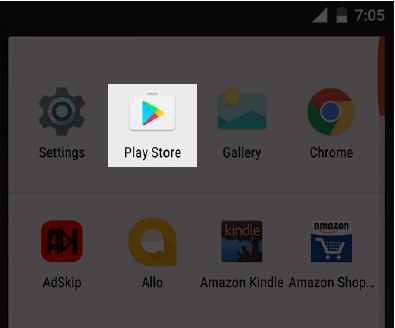
\includegraphics[width=\textwidth]{playstore.png}}

        \end{center}
        In order to use this application on a computer browser, you will need Javascript and Cookies enabled. The steps to enable these, if it is not enabled by default, is outlined on the next page.
        \newpage
        \subsection{Chrome}
            \subsubsection{Enabling Cookies and Javascript}
            \begin{enumerate}
                \item Click the Customize and control Google Chrome icon (three horizontal bars in the upper right corner).
                \item Select Settings.
                \item Click Show advanced settings... at the bottom.
                \item Under Privacy, click the Content Settings button.
                \item Cookies: check Allow local data to be set.
                \item Javascript: check Allow all sites to run JavaScript.
            \end{enumerate}
            \begin{center}
              \makebox[\textwidth]{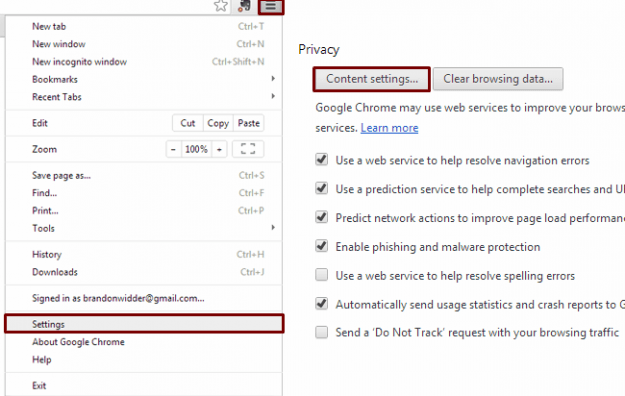
\includegraphics[width=\textwidth]{chromecookies.png}}
            \end{center}
        \newpage
            \subsubsection{Enable Pop-ups}
            \begin{enumerate}
                \item Click the Customize and control Google Chrome icon (three horizontal bars in the upper right corner).
                \item Select Settings.
                \item Click Show advanced settings... at the bottom.
                \item Under Privacy, click the Content Settings button.
                \item In the Pop-up section select Manage exceptions and add our URL : https://unclutter.iminsys.com
                \item Select Allow under Behaviour.
                \item Click Done
            \end{enumerate}
            \begin{center}
             \makebox[\textwidth]{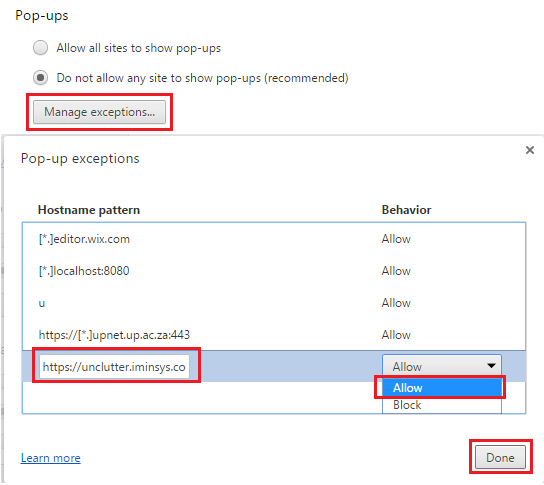
\includegraphics[width=\textwidth]{chromepop.png}}
           \end{center}
            
        \newpage
        \subsection{Firefox}
            \subsubsection{Enable Cookies and Javascript}
            \begin{enumerate}
                \item Click the Firefox menu in the left hand corner of the window.
                \item Select Options.
                \item Click Content.
                \item Check the Enable JavaScript box.
                \item Click Privacy.
                \item Under the History heading, set Firefox will to Remember History.
                \item Click OK.
            \end{enumerate}
            \begin{center}
              \makebox[\textwidth]{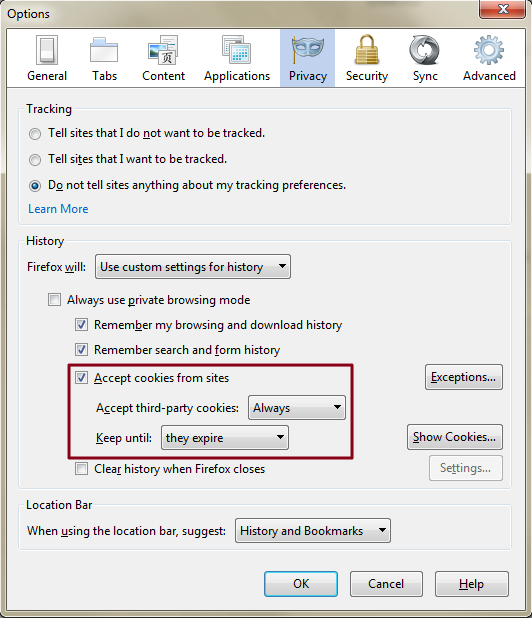
\includegraphics[width=\textwidth]{firefoxcookies.png}}
            \end{center}
        \newpage
            \subsubsection{Enable Pop-ups}
            \begin{enumerate}
                \item Click the Firefox menu in the left hand corner of the window.
                \item Select Options.
                \item Click Content.
                \item Under Pop-ups click Exceptions
                \item Add the URL : https://unclutter.iminsys.com
                \item Click Allow.
                \item Click Save Changes.
            \end{enumerate}
           \begin{center}
              \makebox[\textwidth]{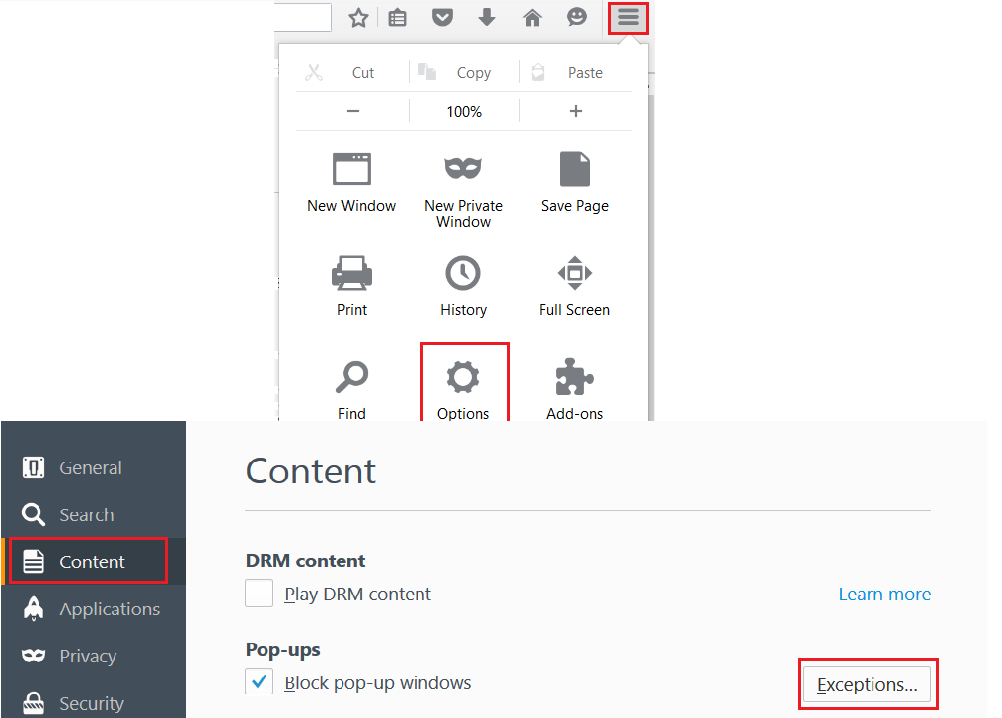
\includegraphics[width=\textwidth]{firefoxpop.png}}
            \end{center}
     
        \newpage
        \subsection{Internet Explorer}
            \subsubsection{Enabling Cookies and Javascript}
            \begin{enumerate}
                \item From the Tools menu, select Internet Options. (In IE9 and up, the Tools menu is a gear icon)
                \item To enable session cookies, click the Privacy tab.
                \item Locate the Settings slider and change the privacy settings to Medium. If you have an older version of IE, locate and click the checkbox next to Always allow session cookies.
                \item To enable JavaScript, click the Security tab.
                \item Under Select a zone to view, click Internet.
                \item Locate the Custom area of the Security tab, and click the Custom Level button.
                \item From the Security Settings dialog box that opens, scroll through the options until you see Scripting.
                \item Check the radio buttons next to Enable Active Scripting and Scripting of Java applets.
                \item Click OK to accept scripting and cookie handling changes and close the Security Settings window.
                \item From the Internet Options dialog box, click Apply to effect settings, and then OK to close the box.
            \end{enumerate}
            \begin{center}
              \makebox[\textwidth]{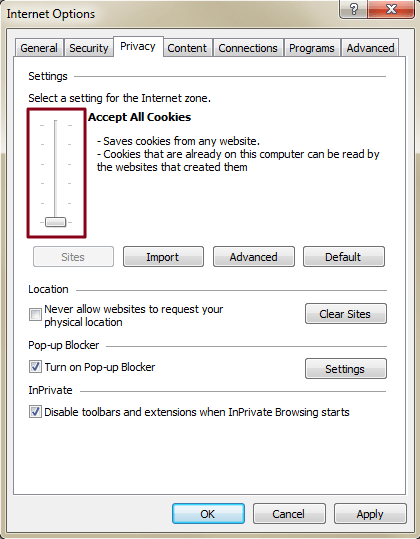
\includegraphics[width=\textwidth]{explocookies.png}}
            \end{center}
            \newpage
            \subsubsection{Enabling Pop-ups}
            \begin{enumerate}
                \item From the Tools menu, select Internet Options. (In IE9 and up, the Tools menu is a gear icon)
                \item Click the Privacy tab.
                \item Under Pop-up Blocker click Settings
                \item Add URL: https://unclutter.iminsys.com click Add then Close.
                \item In Microsoft Edge click settings
                \item Scroll down and click View advanced settings
                \item Click the Block pop-ups so it changes to off
                
            \end{enumerate}
            \begin{center}
              \makebox[\textwidth]{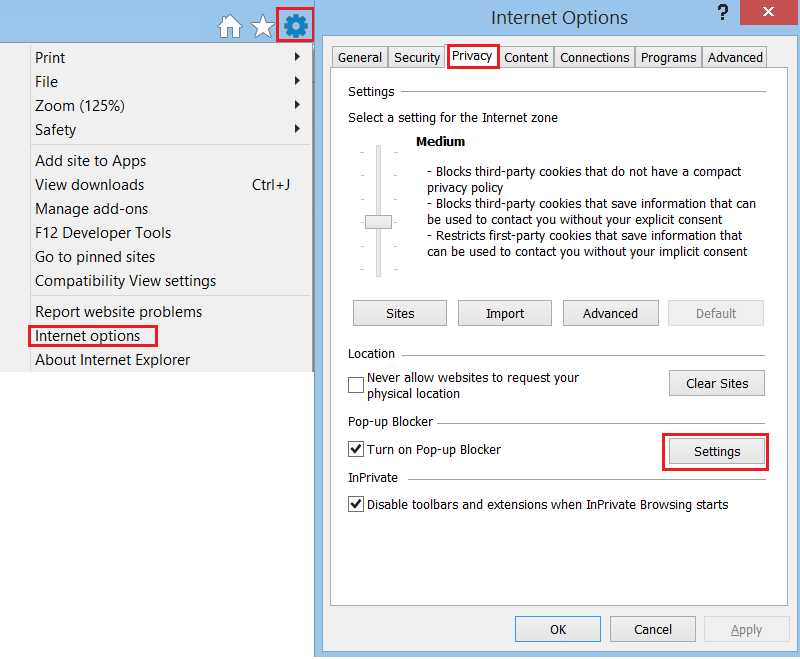
\includegraphics[width=\textwidth]{explopop.png}}
            \end{center}
        \newpage
        \subsection{Safari}
        \subsubsection{Enabling Cookies and Javascript}
            \begin{enumerate}
                \item Click Safari in the menu bar and choose Preferences.
                \item From the Preferences dialog box that opens, select the Security option.
                \item Under Web Content, check the Enable JavaScript box.
                \item Select the Privacy option.
                \item Make sure Block Cookies is not set to Always.
            \end{enumerate}
            \begin{center}
              \makebox[\textwidth]{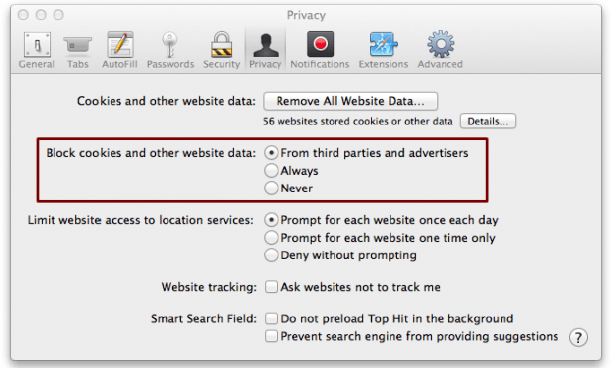
\includegraphics[width=\textwidth]{safaricookies.png}}
            \end{center}
         \subsubsection{Enabling Pop-ups}
            \begin{enumerate}
                \item Click Safari in the menu bar and choose Preferences.
                \item From the Preferences dialog box that opens, select the Security option.
                \item Ensure the Block pop-up option is not checked i.e. uncheck it to allow pop-ups
            \end{enumerate}
            \begin{center}
              \makebox[\textwidth]{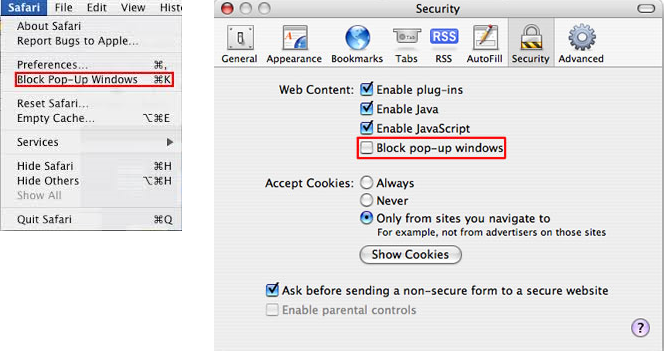
\includegraphics[width=\textwidth]{safaripop.png}}
            \end{center}
        \subsection{Security}
            Some risks associated with enabling Javascript and/or cookies are Session Hi-jacking, XSS, CSRF and Cookie stealing. However, most of these risks can be circumvented by using an up-to-date browser. Other threats, like CSRF(cross site request forgery) are handled on our server side.
    \section{Configuration} 
        \begin{center}
          \makebox[\textwidth]{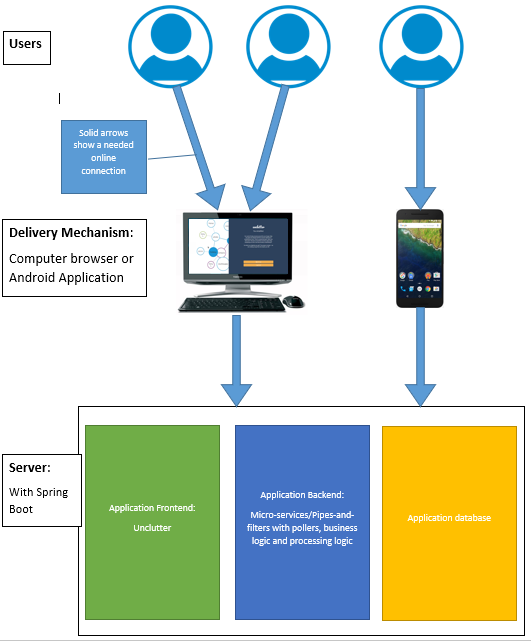
\includegraphics[width=\textwidth]{config.PNG}}
          Hardware needed: A touch screen device or a computer with a mouse and keyboard. Device needs to be connected to the Internet.
          \label{Config}
        \end{center}

        
    \section{Getting started}
        \paragraph\indent
        Since this is an application that heavily relies on the user interface and the user experience, we have put much emphasis on how our application looks, feels and response to the user. We tried to keep in mind that not all users have good computer skills and thus our approach was to make the interface as user friendly as possible, with clear buttons and directions on how to use the system while they are using it.
    \subsection{Mobile}
            \paragraph\indent
            Unclutter was developed for desktop browsers, but is mobile compatible, resizing components and interfaces to fit any screen. Any interface shown in this manual can be applied to both desktop and mobile platforms and a mobile representation will often be shown in this document as to show the usability of the systems interface on any platform or screen size. An Android application has also been developed and looks and feels the same as if it were run in the mobile browser. Therefore any reference to \textit{mobile} includes the Android application.
        
    \subsection{Landing Page}
        First navigate to the link \url{https://unclutter.iminsys.com/}. Here you will see a landing page showing the user a short abstract of what the system is about. Here they can choose to login if they already have an account or register a new account. If a user tries to login a account without registering, they will be directed back the the landing page with a message to tell them they aren't registered on the system and to please register first.
        \begin{center}
          \makebox[\textwidth]{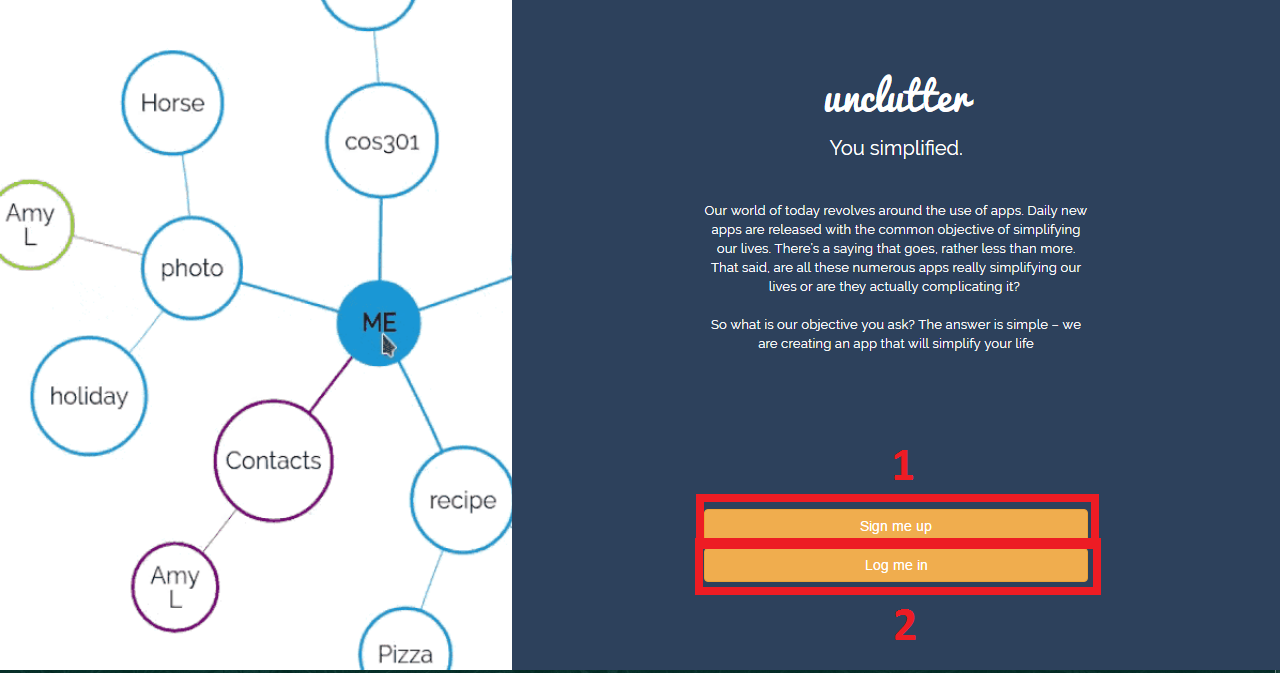
\includegraphics[width=\textwidth]{landing.PNG}}
          Figure 1: Landing page.
          \label{Landing Page}
        \end{center}
        \begin{enumerate}
            \item This button will lift up the landing page and show the register page underneath. Clicking the back button on the register page will show the landing page again.
            \item This button will lift up the landing page and show the login page underneath. Clicking the back button on the login page will show the landing page again.
        \end{enumerate}
        \newpage
        
    \subsection{Log In}
            After clicking the \textit{Log me in} button the log in page will load, looking like this:
            \begin{center}
              \makebox[\textwidth]{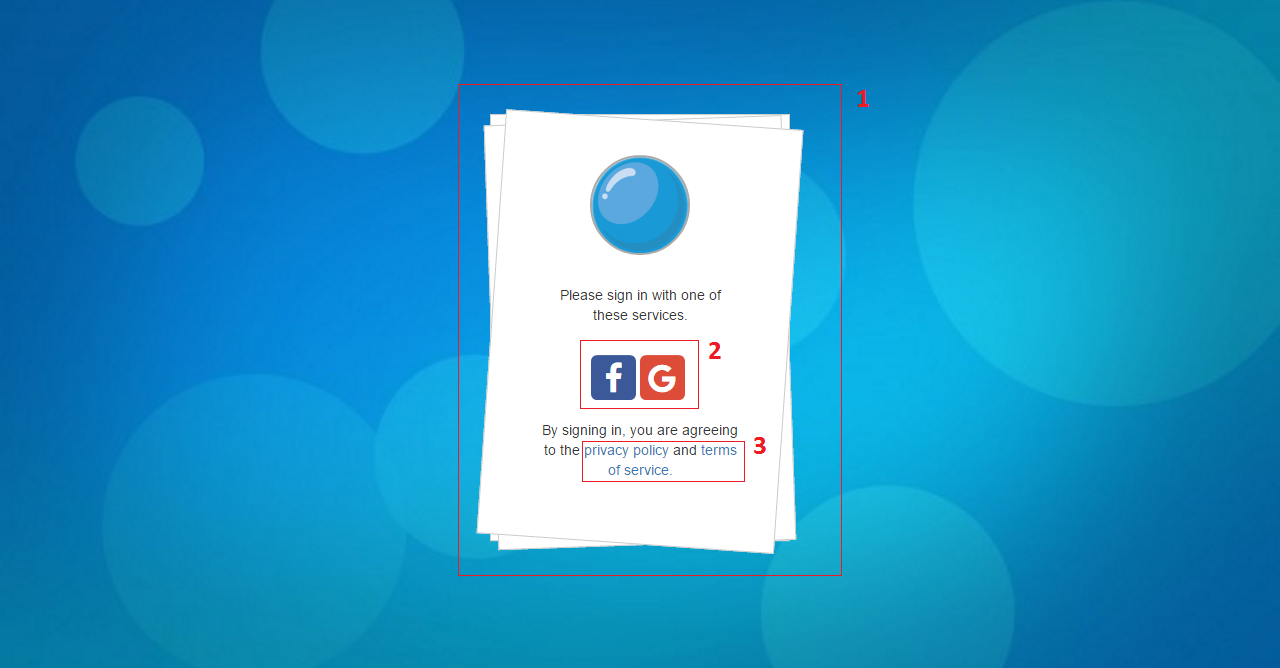
\includegraphics[width=\textwidth]{login.PNG}}
              Figure 2: Initial log in screen.
              \label{Log In}
            \end{center}
        \begin{enumerate}  
            \item If the user tries and access the main page any other way than logging in the will be redirected back here to the log in page. 
            \item The user may log in either through clicking and signing in with the Facebook button or the Google button using the respective user credentials of either system. We do not store any user credentials on our system.
            \item Before logging in the user may view our privacy policy or terms of service. 
        \end{enumerate}
        
        After a successful log in a  message will be show and a continue button which will take us to the home page.
        \begin{center}
          \makebox[\textwidth]{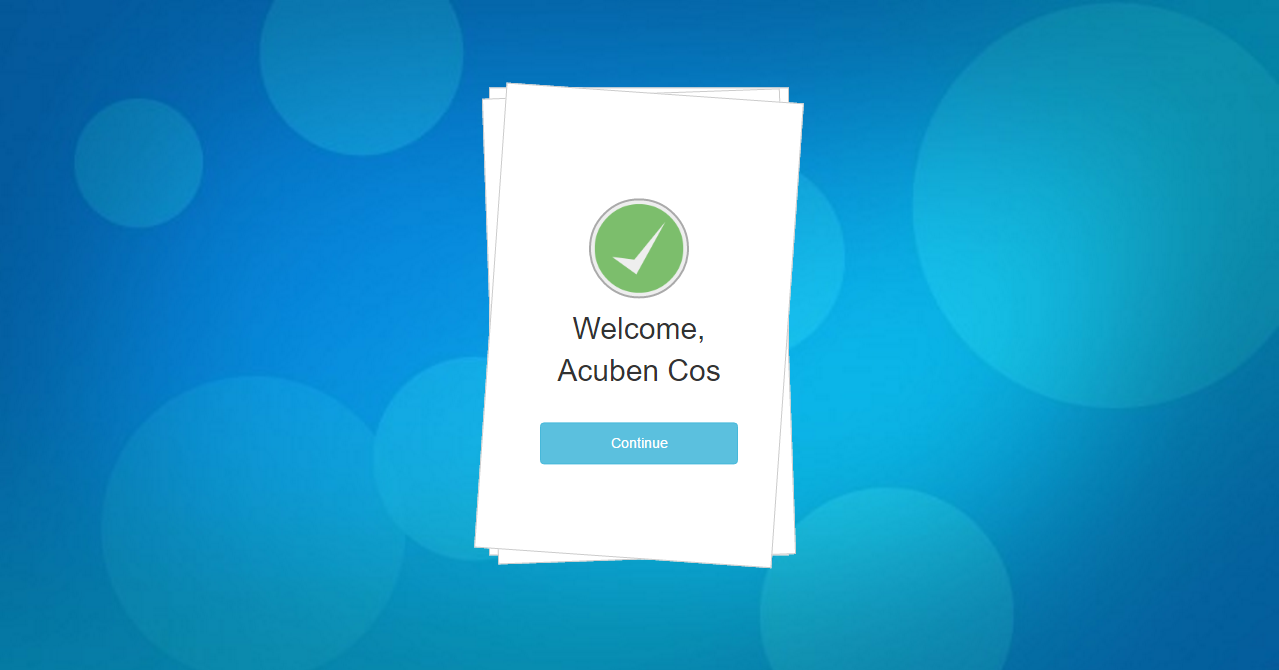
\includegraphics[width=\textwidth]{login2.PNG}}
          Figure 3: Success log in screen.
          \label{Log In Success}
        \end{center}
        
    \subsection{Register}
        If a user clicks on the \textit{Sign me up} button, the register page will load and we will see a screen that contains multiple buttons each with labels of social media or "data sources" where the system will extract data from to build a mind map on the home page for the user. More than one data source can be selected. Data sources include social media such as Google and Facebook.
        \begin{center}
          \makebox[\textwidth]{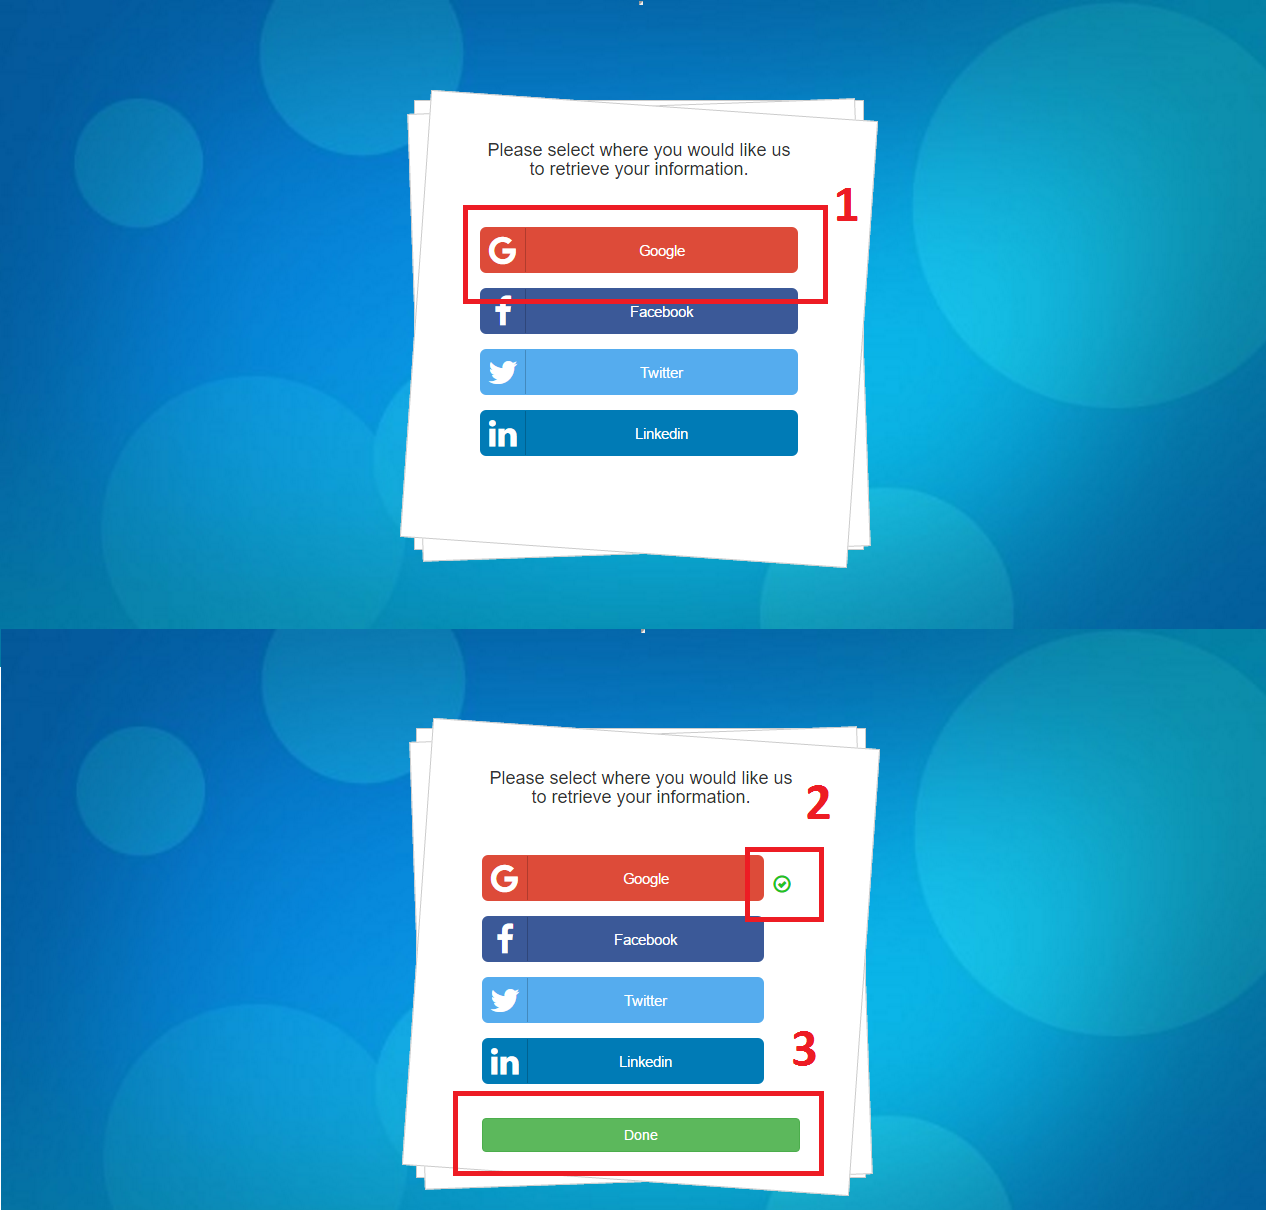
\includegraphics[width=\textwidth]{selectdata2.PNG}}
          Figure 4: Selecting data sources to display on mindmap.
          \label{Select Data}
        \end{center}

        \begin{enumerate}  
            \item First the user should select what data source they would like to retrieve data from. As soon as the user selects the Google button then Google will ask you permission to grant the application access.
            \item After Google has granted the system access, a tick will show next to the respective data source to show we have successfully processed the request. The user may now choose another data source like Facebook.
            \item When the user is satisfied with the data sources they would like to use, they can proceed to click on the "Done" button. Note: a user may select more than one. This will request the server to start the building of the mind map and to create the main page for the user. While this is happening a "Loading..." message will show on the bottom left hand side. Please be patient here as this step relies on your Internet connection. After a successful request, the user will be redirected to the next page.
        \end{enumerate}
    \subsection{Help Page}
        While the system is retrieving topics, a help page will be displayed to the user to show them how to use the system and when the system is ready, we will display a button for them to move to the next page.
        \begin{center}
            \makebox[\textwidth]{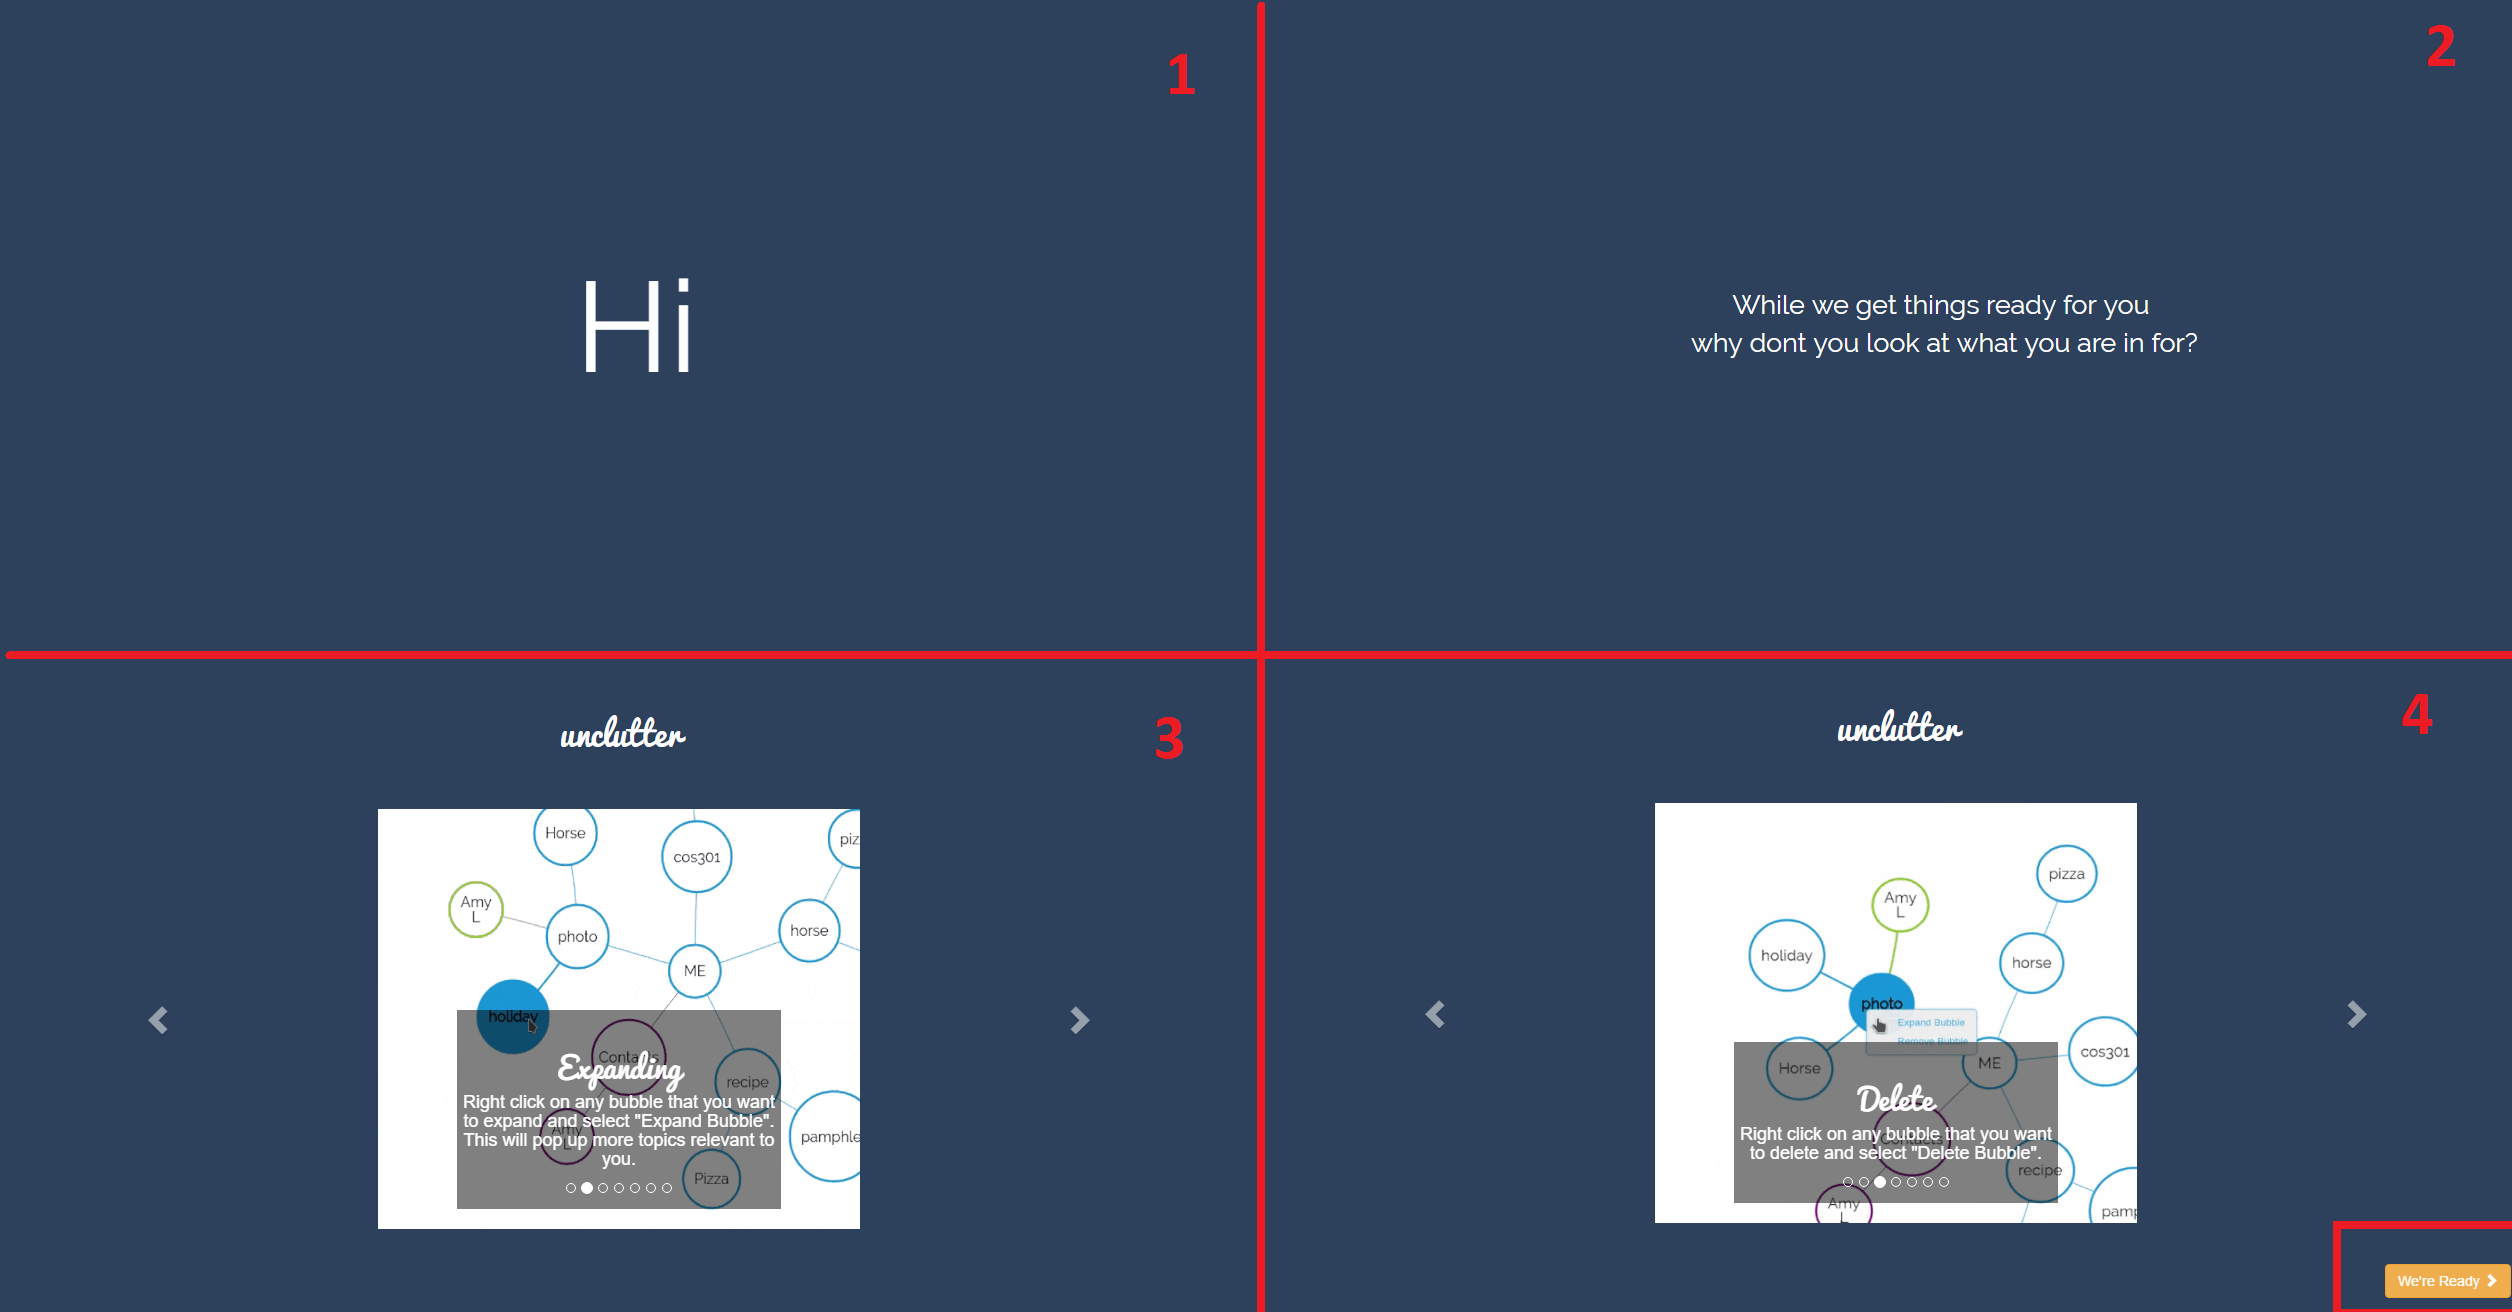
\includegraphics[width=\textwidth]{help.PNG}}
          Figure 5: Help screen.
          \label{Help}
        \end{center}
        
    \section{Using the system}
    \subsection{Home Page}
    When the user is redirected they will be greeted with a lonely "ME" bubble, a navigation bar that has "Help", "Settings","Log out" buttons and a message on the bottom left saying "loading...". This is the part where the back end is processing the new data and sending it the the mind map. Please be patient as this step is reliant on your internet connection. After everything has been successfully initialised and processed, the first few bubbles with topics most relevant to the user will pop up around the me bubble. The graph is highly interactable, with each bubble having the ability to be moved, selected, double tapped and right clicked on, each of which give you a different action, all explained below. 
    \begin{center}
      \makebox[\textwidth]{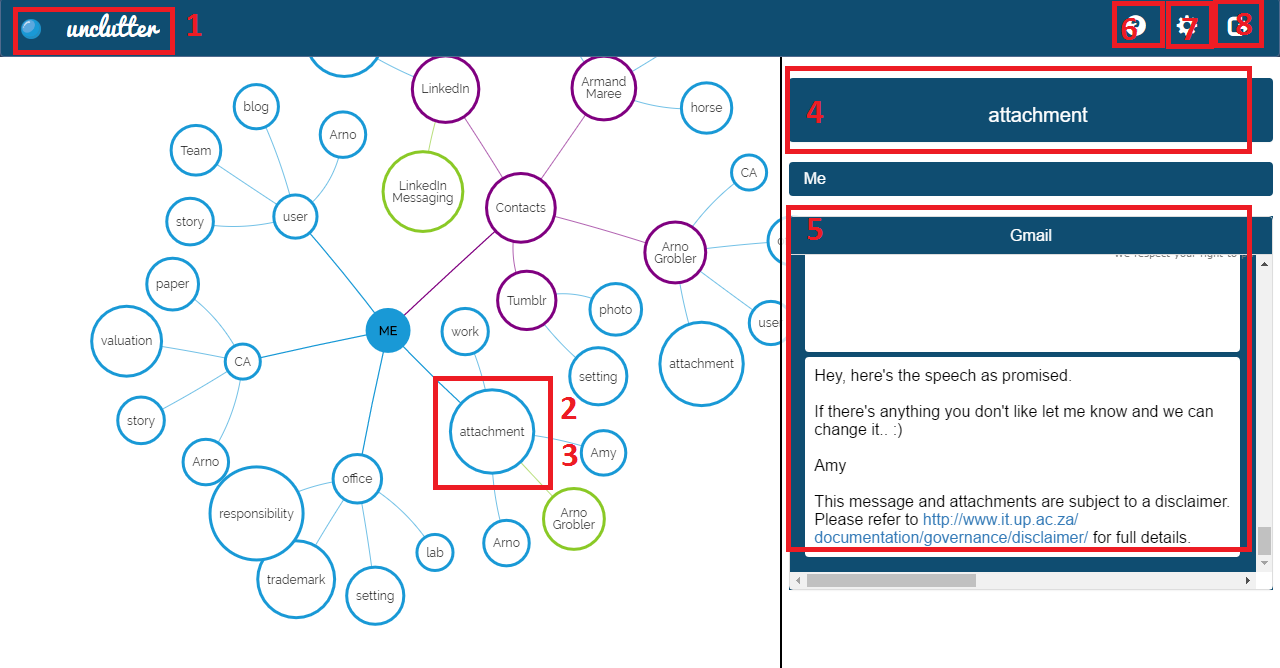
\includegraphics[width=\textwidth]{main.PNG}}
      Figure 6: Main Page with loaded bubbles, right click menu deactive and side bar open with Gmail option expanded.
      \label{Main page}
    \end{center}
    \begin{enumerate}  
        \item Here we see the logo of unclutter. It doubles as a home button to easily get back to the home page and a back button shown later in the mobile view when the side bar is activated.
        \item This is what is referd to as a "Bubble". It is a node of the mind map showing a particular topic of relevance to the user. The system chooses the particular topics from your actual data you specified when you selected the data sources. The further down the path the particular bubble is from the "ME" bubble, the less relevant it is. When you expand a bubble, all the bubbles around it will be relevant to both the selected bubble and the path it follows from the "ME" bubble, where the path is shown in number 4 below. A bubble can be right clicked to bring up a context menu(3), left clicked to be selected and moved and double clicked to bring up a side bar.
        \item This is the context menu, created when the user right clicks a bubble. There is two options present to the user at the moment: "Expand Bubble" and "Delete Bubble". When you expand a bubble, all the bubbles around it will be relevant to both the selected bubble and the path it follows from the "ME" bubble, where the path is shown in number 4 below. When you delete a bubble, the currently selected bubble will be deleted and all the connected bubbles around it. Each bubbles colours mean something different: If it is blue it means it is a topic, if it is green it is a related contact and purple means it is part of the \textit{quick access contacts}.
        \item This is the breadcrumb path of the currently selected bubble from the "ME" bubble. It is shown when a user activates the side bar by double clicking on the node they want more info about. The side bar will also contain the actual data about that topic that was selected in (5) shown below.
        \item This is the actual data about that topic that was selected. This includes the actual Gmail emails and Facebook posts the server used to process to get the relevance of the selected node. Later functionality will be added to be able to reply to these emails directly from the side bar.
        \item This button is the "Help" button and will redirect the user to the help page discussed previously
        \item This is the Settings button. It expands to a drop down that gives a few options  and a " Account Settings" option where the user will be redirected to a settings page where they can change user preferences (discussed below).
        \item This is the Log out button. It will log the user out of its current session and redirect the user to the log in page
        \item This is the view of the Home Screen viewed on a mobile device. Below three screens are shown, first a default screen with nothing selected, then a screen where the options hamburger button is clicked on the top right hand corner in the navigation bar, and lastly the view if the user double clicks on the holiday bubble, giving the user an option to go back on  the left top hand corner
    \end{enumerate}
    \begin{center}
      \makebox[\textwidth]{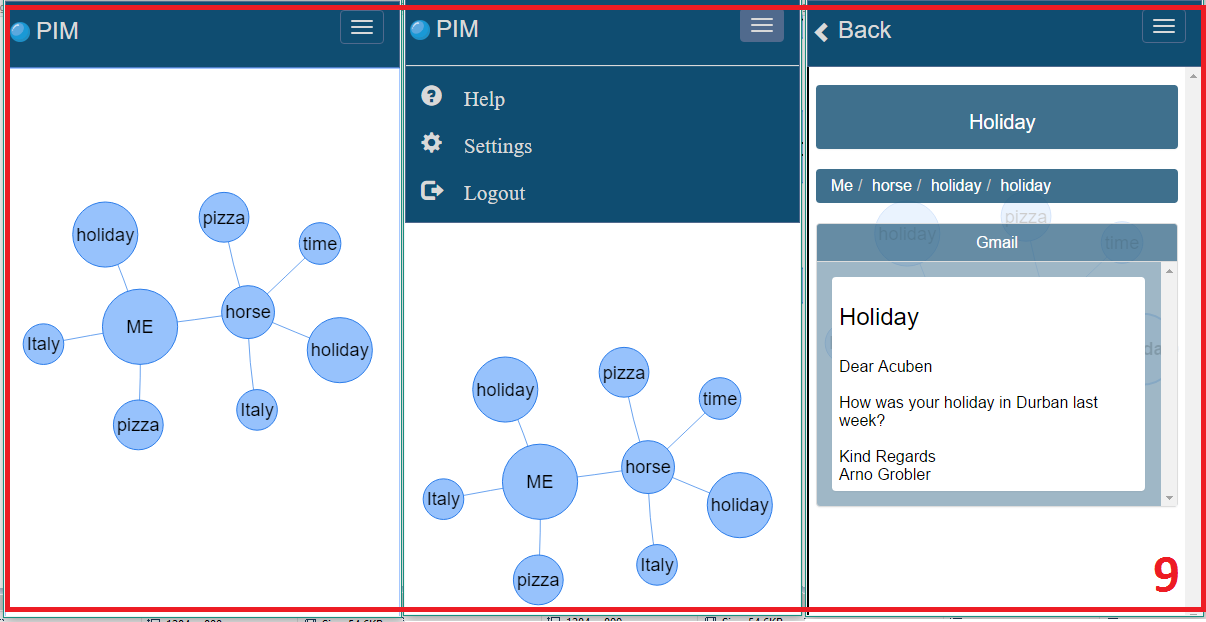
\includegraphics[width=\textwidth]{mobile1.PNG}}
      Figure 7: Main Page viewed with mobile device with a default unselected bubble screen, a opened options menu screen and a selected bubble screen.
      \label{mobile page}
    \end{center}
    \subsection{Settings}
        After clicking on the \textit{Account Settings} button on the main page, you will be directed to the settings page where you will find a tabbed panel with three tabs: Account, Theme and User preferences. All are expanded below
     \begin{center}
      \makebox[\textwidth]{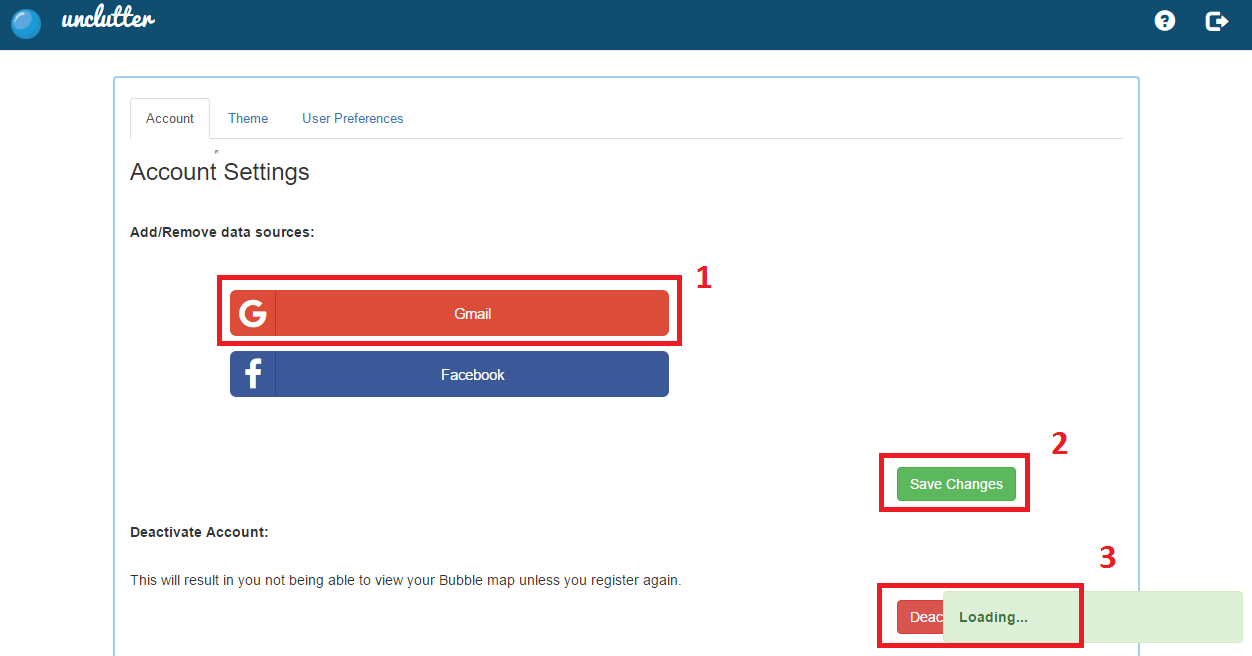
\includegraphics[width=\textwidth]{settings1.PNG}}
      Figure 9: Settings page with \textit{Account} tab open. 1) here you can select and deselect data sources. 2) After you have made your changes, click this button to save the changes. 3) Deactivate your account wit this option.
      \label{settings page 1}
    \end{center}
    \begin{center}
      \makebox[\textwidth]{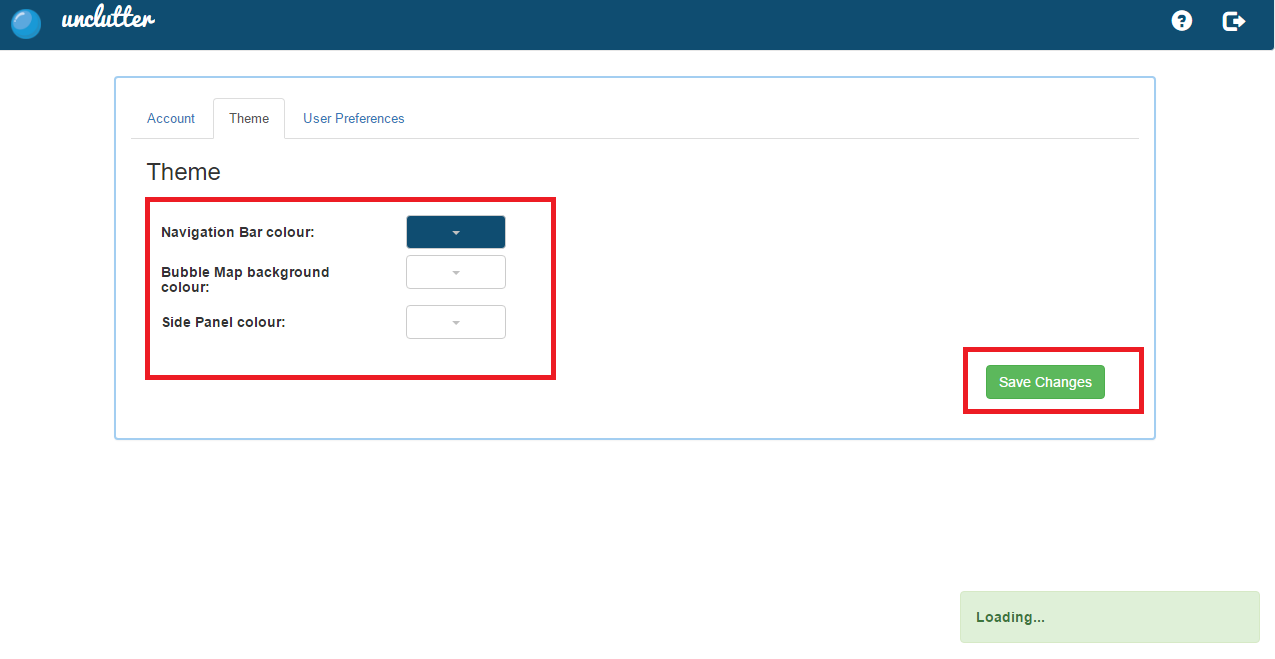
\includegraphics[width=\textwidth]{settings2.PNG}}
      Figure 10: Settings page with the \textit{Theme} tab open. Select what colour you would like the navbar, BubbleMap background and sidebar to be and then click save
      \label{settings page 2}
    \end{center}
    \begin{center}
      \makebox[\textwidth]{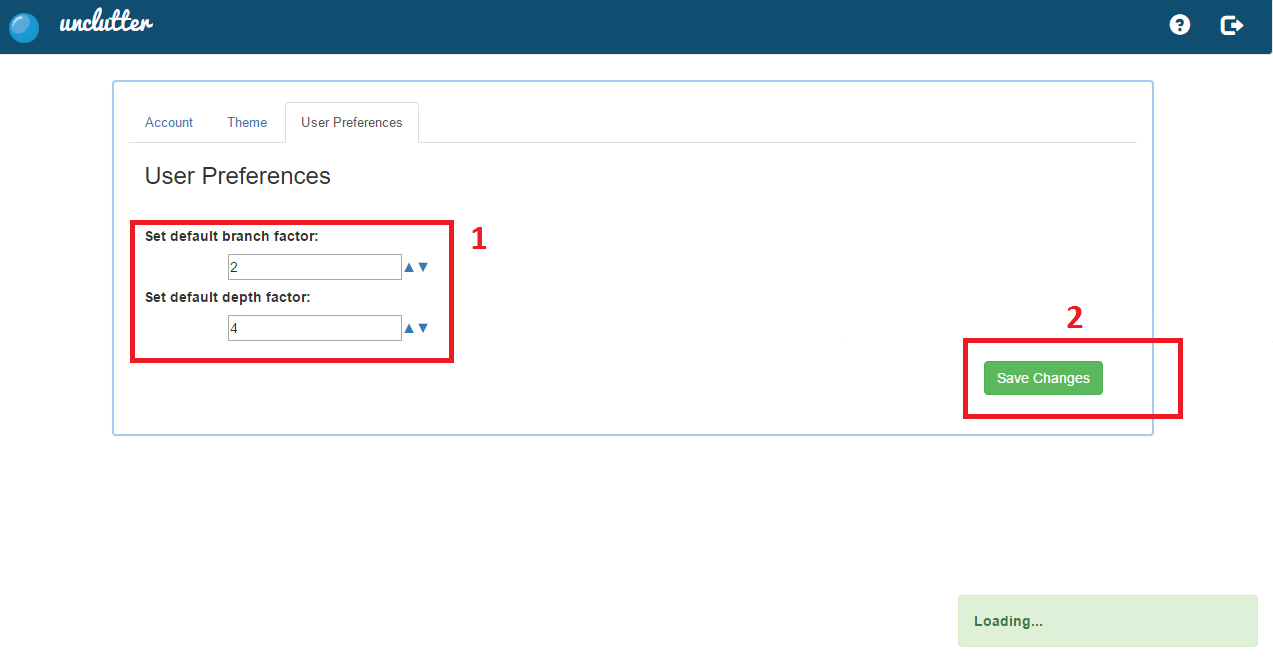
\includegraphics[width=\textwidth]{settings3}}
      Figure 11: Settings page with \textit{User Preferences} tab open. Select you desired depth and branching factor and click save
      \label{settings page 3}
    \end{center}
    
    \section{Troubleshooting}
    Since we handle all errors and problems on our side, the user will never really need to troubleshoot. If something does go wrong, we will let the user know through a message popup (for example if the users internet connection is down, or if they lost connection to our backend) but the only corrective procedure we would require from the user would be to refresh the page. 
\end{document}
 
